\documentclass{beamer}

\usetheme{Warsaw}

\title{How to use \LaTeX}
\author{Andrew McGlathery}
\date{\today}

\begin{document}
  \frame{\titlepage}

\begin{frame}
  \frametitle{What is \LaTeX?}
  \begin{itemize}
    \item A document preperation system
    \item A way to write good-looking papers in your favorite text editor
    \item A turing complete programming language
  \end{itemize}
\end{frame}

\begin{frame}
  \frametitle{Why learn \LaTeX?}
  \begin{itemize}
    \item It is the best way to typeset math
    % put math example here
    \item Conferneces and journals (and upper level classes) require you to submit in \LaTeX
    \item You can write papers and presnetations in your favorite text editor
  \end{itemize}
\end{frame}

\begin{frame}[fragile]
  \frametitle{How to write a simple document}
  Start with the documentclass tag
\begin{verbatim}
\documentclass[12pt]{article}
\end{verbatim}
\end{frame}

\begin{frame}[fragile]
  Next, write your header (this isn't required)
\begin{verbatim}
\title{My Awesome Document}
\author{Andrew McGlathery}
\date{\today}
\end{verbatim}
\end{frame}

\begin{frame}[fragile]
  Finally, write the content of your document
\begin{verbatim}
\begin{document}
  \maketitle
  Cool stuff goes here
\end{document}
\end{verbatim}
\end{frame}

\begin{frame}[fragile]
\begin{verbatim}
\documentclass[12pt]{article}

\title{My Awesome Document}
\author{Andrew McGlathery}
\date{\today}

\begin{document}
  \maketitle
  Cool stuff goes here
\end{document}
\end{verbatim}
\end{frame}

\begin{frame}
  \begin{center}
  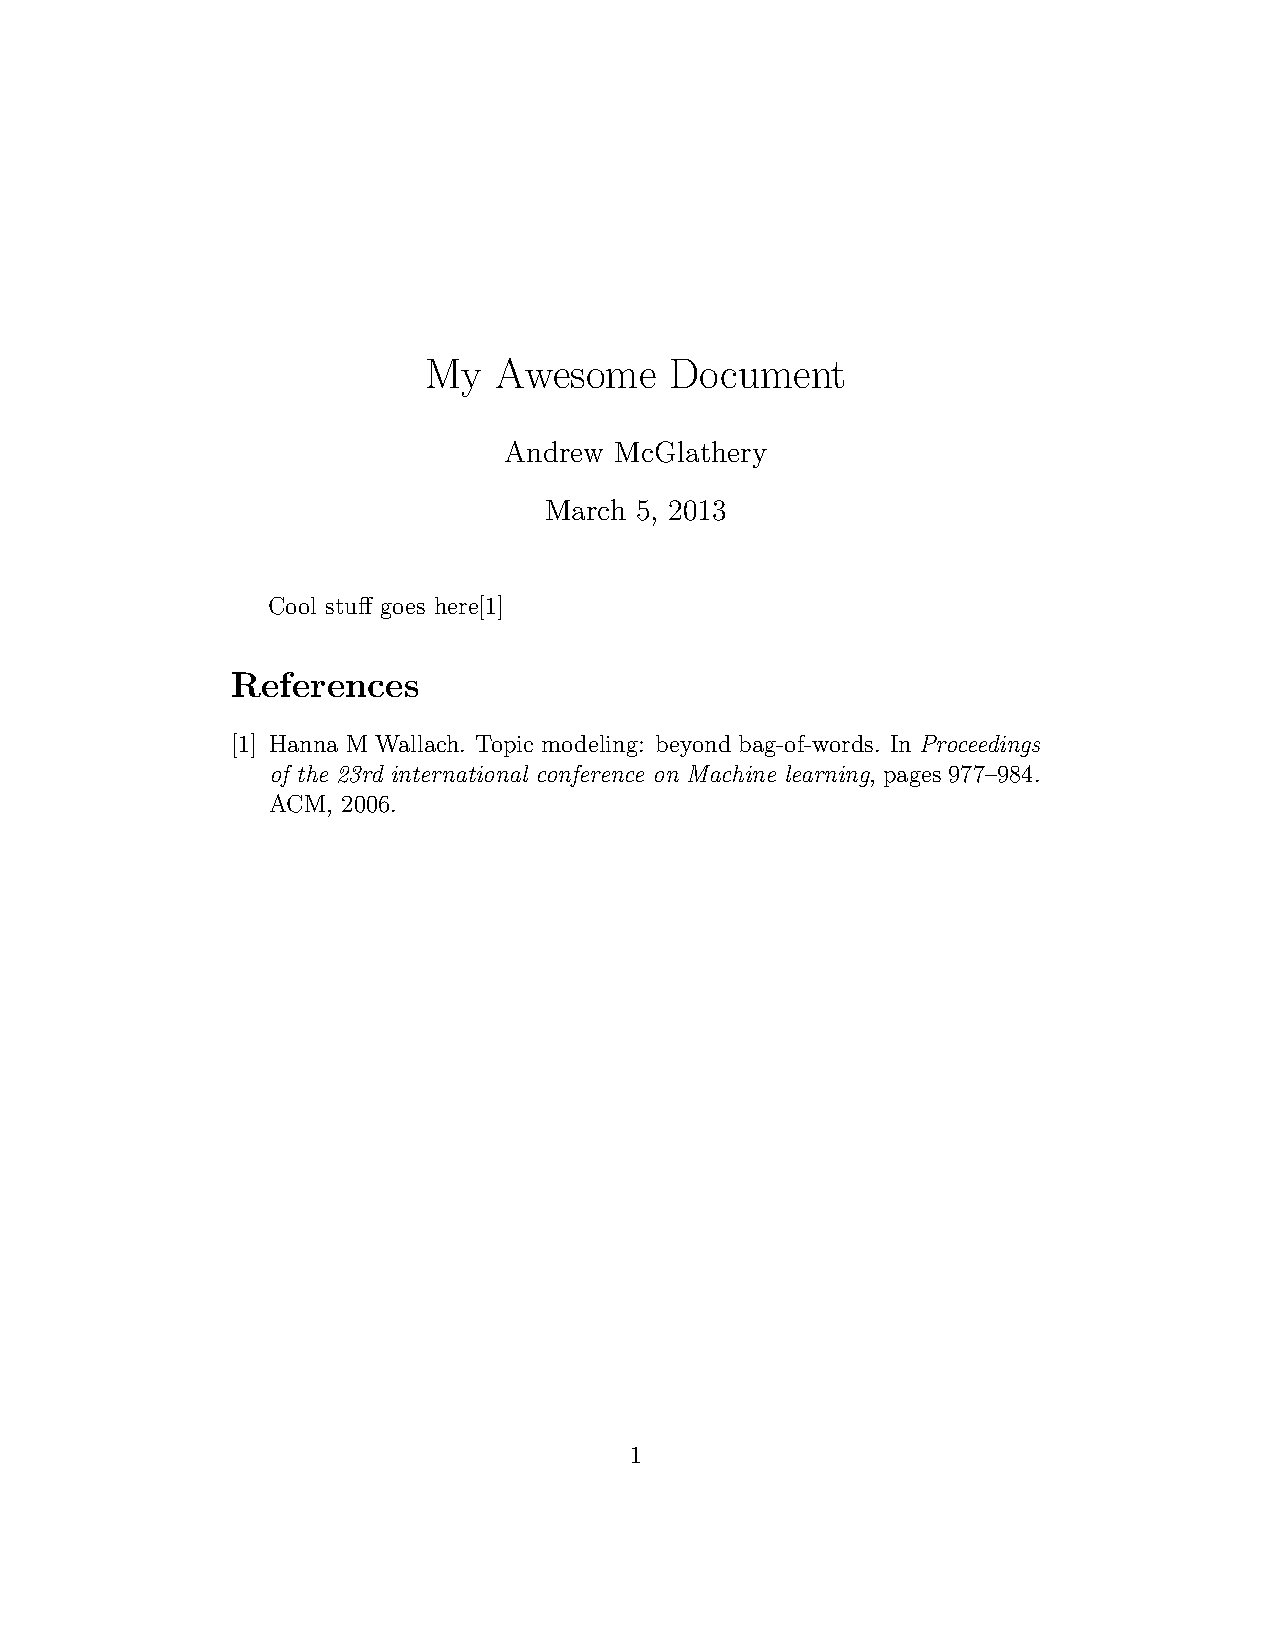
\includegraphics[height=\textheight]{sample_doc.pdf}
  \end{center}
\end{frame}

\begin{frame}
  \frametitle{How do I write math equations in \LaTeX?}
  \begin{itemize}
    \item All inline math is inside of \$ ... \$
    \item All math blocks are inside of \$\$ ... \$\$
  \end{itemize}
\end{frame}

\begin{frame}[fragile]
\begin{verbatim}
Newton's second law is $F=ma$
\end{verbatim}
  Becomes\\
  Newton's second law is $F=ma$
\end{frame}

\begin{frame}[fragile]
\begin{verbatim}
$$
\frac{\frac{y^\alpha}{x_1}+\frac{z_1}{y_2}}{y-z}
$$
\end{verbatim}
  Becomes\\
$$
\frac{\frac{y^\alpha}{x_1}+\frac{z_1}{y_2}}{y-z}
$$
\end{frame}

\begin{frame}[fragile]
\begin{verbatim}
$$
\alpha, \beta, \gamma, \Gamma,
\pi, \Pi, \phi, \varphi, \Phi
$$
\end{verbatim}
$$
\alpha, \beta, \gamma, \Gamma,
\pi, \Pi, \phi, \varphi, \Phi
$$
\end{frame}

\begin{frame}
  \frametitle{Other really cool things in \LaTeX or other things I could talk about}
  \begin{itemize}
    \item Bibtex
    \item GNUplot
  \end{itemize}
\end{frame}

\end{document}
